This section describes the hardware platform used in the experiments. The experiments were conducted on a Texas Instruments TMS320C6678 multi-core digital signal processor. First, the selection of the TMS320C6678 as the hardware platform for the experiments in this thesis is explained in subsection~\ref{subsec:selection-of-platform}. Second, an overview of the hardware platform is given in subsection~\ref{subsec:hw-overview}. After the overview, the key features of the platform are described in subsections \ref{subsec:c66x} C66x DSP, \ref{subsec:c66memory} Memory Hierarchy and \ref{subsec:multicorenav} Multicore Navigator.

\subsection{Selection of the Hardware Platform}
\label{subsec:selection-of-platform}
This thesis investigates stream processing with Open Event Machine on a multi-core DSP. The Texas Instruments Keystone I family of multi-core DSPs has an advanced support for multi-core programming, including a Texas Instruments implementation of OpenEM~\cite{MCSDKbrochure}. The multi-core programming support has not always been a design priority of multi-core DSPs, for example the TMS320C647x DSPs were looked at as, "multiple single-core DSP in a single package" by the programmers~\cite{moerman2014open}.

The hardware platform used in the experiments in this thesis is the Texas Instrument TMS320C6678. The TMS320C6678 is a fixed and floating point digital signal processor based on the Texas Instruments Keystone I architecture~\cite{tmsdatasheet}. The Keystone I architecture was selected because there exists an OpenEM implementation for that supports the processors implementing the architecture. Out of the Keystone I devices TMS320C6678 was selected because Advantech provides an evaluation module TMDXEVM6678L for the specific processor, which makes the experimentation more straightforward than building an evaluation platform from scratch. Another benefit of the TMS320C6678 is that the PREESM rapid prototyping tool for dataflow applications has support for it~\cite{pelcat2014preesm}.

\subsection{TMS320C6678 Overview}
\label{subsec:hw-overview}

\begin{figure}[h!]
    \begin{center}
        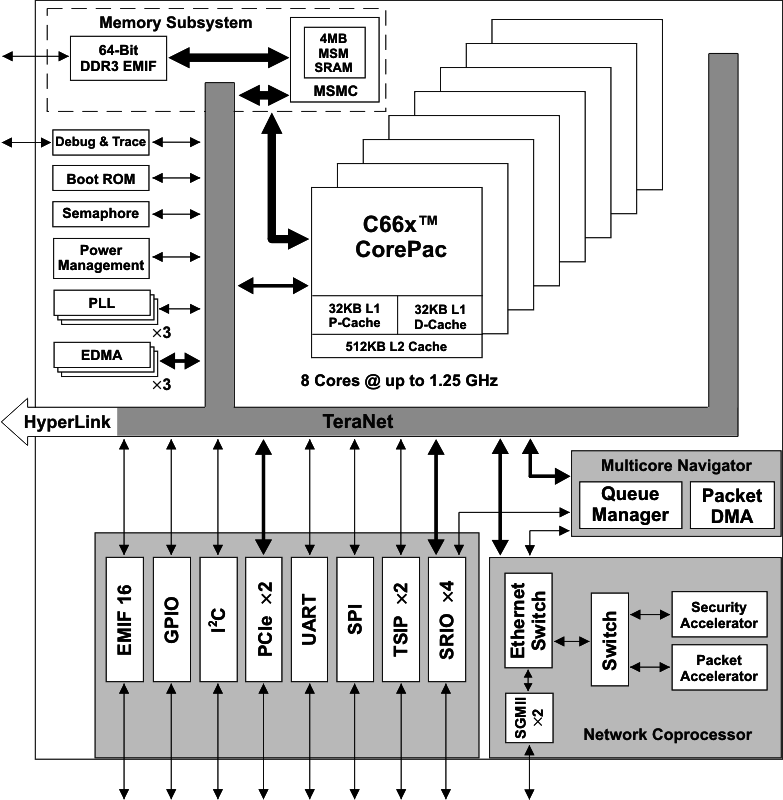
\includegraphics[width=0.99\textwidth]{images/fbd_SPRS691e.png}
        \caption{High-level schematic of the TMS320C6678 architecture. Figure from~\cite{tmsdatasheet}.}
        \label{fig:arch_overview}
    \end{center}
\end{figure}

The TMS320C6678 is based on the Keystone I architecture. The Keystone I architecture specifies a set of hardware elements which enable integration of C66x DSP cores, application specific co-processors and IO \cite{tmsdatasheet}. The Keystone I hardware modules and their connections are presented in the figure \ref{fig:arch_overview}. The points of interest in the figure in the scope of this thesis are the C66x CorePac cores depicted in the middle of the figure, the memory subsystems and its components in the top-left of the figure and the Multicore Navigator depicted in the right edge of the figure.

In the Keystone I architecture there are multiple ways for the C66x cores to communicate with each other, the memory and the peripherals. The methods of communication of specific interest for the experiments in this thesis are communication through shared memory discussed in subsection \ref{subsec:c66memory} and communication through packet based communication manager Multicore Navigator introduced in subsection \ref{subsec:multicorenav}.

The development board used for development of the experiment applications and measurements is an Advantech TMDXEVM6678L. TMDXEVM6678L is an evaluation module for the TMS320C6678 multi-core DSP. The evaluation module has 512 megabytes of DDR3 memory which is sufficient for stream processing applications. Another important feature of the evaluation module is the emulator module with USB connectivity. The emulator together with the Code Composer Studio IDE (CCS) make the programming and debugging the experiment programs for the DSPs uncomplicated.~\cite{evmref} CCS version 5.2 is distributed with the hardware evaluation module and was used for development of the experiments in this thesis.

\subsection{C66x DSP}
\label{subsec:c66x}
The hardware platform used in this thesis is the TMS320C6678. The TMS320C6678 consists of eight C66x DSP cores. The C66x is based on the Texas Instruments TMS320C66x instruction set architecture. The TMS320C66x is a very long instruction word architecture, which allows for high amount of instruction level parallelism. The C66x has a total of eight functional units, which operate in parallel. This means that the C66x can dispatch up to eight instructions per cycle. The instructions dispatched in parallel move through pipeline stages simultaneously. Pipelining helps eliminate CPU stalls while waiting for memory operations or other CPU instructions taking multiple cycles complete.~\cite{sprugh7}

Keeping the utilization of the wide pipeline high, the CPU needs to have enough registers to prevent excessive memory access stalling. The CPU has 64 32-bit general purpose registers~\cite{sprugh7}. The C66x is a high-end processor with native support for 32-bit and 64-bit floating point instructions and capability of clock speeds up to 1.4 GHz~\cite{sprugh7}.

\subsection{Memory Hierarchy}
\label{subsec:c66memory}
The TMS320C6678 contains a multi-layer memory hierarchy which can be configured by the user to a large extent. The memory hierarchy in the device consists of L1 and L2 memories for each core, Multicore Shared Memory (MSM) and additionally external memory provided by the evaluation module. In the figure~\ref{fig:arch_overview} the memories are placed inside the subsystems they are part of, MSM can be found in the upper-left corner as part of the memory subsystem.

Each c66x CPU has 32 KB level 1 program cache (L1P), 32 KB level 1 data cache (L1D). Each CPU also has 512 KB of level 2 cache. Both of the L1 caches and the L2 cache can be found in the figure~\ref{fig:arch_overview} as part of the C66x CorePac box. Initially after bootup both L1P and L1D are configured as cache but they can be reconfigured as addressable memory by software. The L2 memory is always configured as addressable memory after reset but can be configured as cache by software. \cite{tmsdatasheet} L2 SRAM addresses are always cached with L1P and L1D whereas external memory addresses are configured noncacheable by default~\cite{cacheguide}.

Configuring the state of the L1 and L2 memories as well as other memory configurations can be handled with software \cite{sprugh7}. CCS automatically handles a lot of the memory mapping needed for applications and provides tools for creating custom configurations.

In PC hardware cache coherence is usually handled automatically by the hardware. In c66x, however, that is not the case. Each c66x core maintains cache coherence between its L1 caches and the L2 cache automatically but programmer needs to manage coherence in most other cases. For example if caching is enabled for an external memory region shared by two cores, explicit cache coherence operations need to be performed before each core can read from or write to the shared region~\cite{cacheguide}.

The evaluation module has 512 MB of DDR3 memory \cite{evmref}. The memory in the evaluation module, as any external memory in other hardware configurations, is accessible through the Multicore Shared Memory Controller (MSMC). The MSMC itself contains 4096KB of shared memory accesible by all cores. In the figure~\ref{fig:arch_overview} the memory subsystem contains the EMIF link to the external memory and the MSMC.

\subsection{Multicore Navigator}
\label{subsec:multicorenav}
The multi-core programmability of the TMS320C6678 makes it interesting for this thesis. The device is designed to allow simple co-operation of the DSP cores and provides the required hardware support for that purpose. The core features enabling the multi-core programmability are grouped under the name of Multicore Navigator.

Multicore Navigator is the name for a collection of features in Keystone I and II devices, which enables hardware-accelerated, packet-based communication between on-chip devices. Texas Instruments claims the use of specialized hardware for on-chip communication results in significant performance gains when implemented carefully. The design goals stated for the Multicore Navigator in \cite{navigator} are minimizing host interaction and maximizing memory use efficiency.~\cite{navigator}

In Keystone I devices such as the TMS320C6678, the Multicore Navigator provides a hardware queue manager, a special direct memory access for different subsystems called Packet DMA (PKTDMA), and multi-core host notifications via interrupts. \cite{navigator} The Texas Instruments OpenEM implementation \ref{chapter:openem} heavily utilizes the features provided by Multicore Navigator.

The Queue Manager on Keystone I architecture devices is a hardware module that manages 8192 queues. Packets are queued and dequeued from the queues by the applications. The Queue Manager is responsible for accelerating the packet communication. In addition to the Queue Manager the Queue Management Subsystem contains two Packed Data Structure Processors (PSDP) which perform tasks related to the queue management and packet communication. For example the PDSP processors can be used to perform accumulation of packets. The accumulation program is given a list of queues to poll. Whenever it finds a descriptor from one of the queues it is watching it will pop the descriptor and place it in a buffer provided by the application. After a pre-determined number of descriptors, or after reaching its time limit, the accumulator program notifies the host processor about the descriptors in the buffer via an interrupt. Use of such firmware offloads the burden of queue polling from the host processors.~\cite{navigator} The TI implementation of OpenEM \ref{chapter:openem} provides its own firmware for the PDSP cores which is utilized by the OpenEM runtime for event scheduling \cite{moerman2014open}.

The PKTDMA is a special DMA utilized by the Multicore Navigator to transfer packet buffers between memory locations. When a packet is sent to a queue The PKTDMA reads the address of the data to be transferred from packet descriptor, transfers the data in one or more data moves and writes the pointer to the data queue specified as the receiver of the packet. The PKTDMA is useful because it allows the program running on a PDSP core to move data in the memory without interrupting the host processors.~\cite{navigator} OpenEM uses PKTDMA to move event buffers to the caches of the core, which is about to receive the event~\cite{moerman2014open}.
